\section{Auswertung}
\label{sec:Auswertung}
\subsection{Dämpfung des elektischen Schwingkreises}
\label{sec:dae}
\begin{figure}[H]
  \centering
  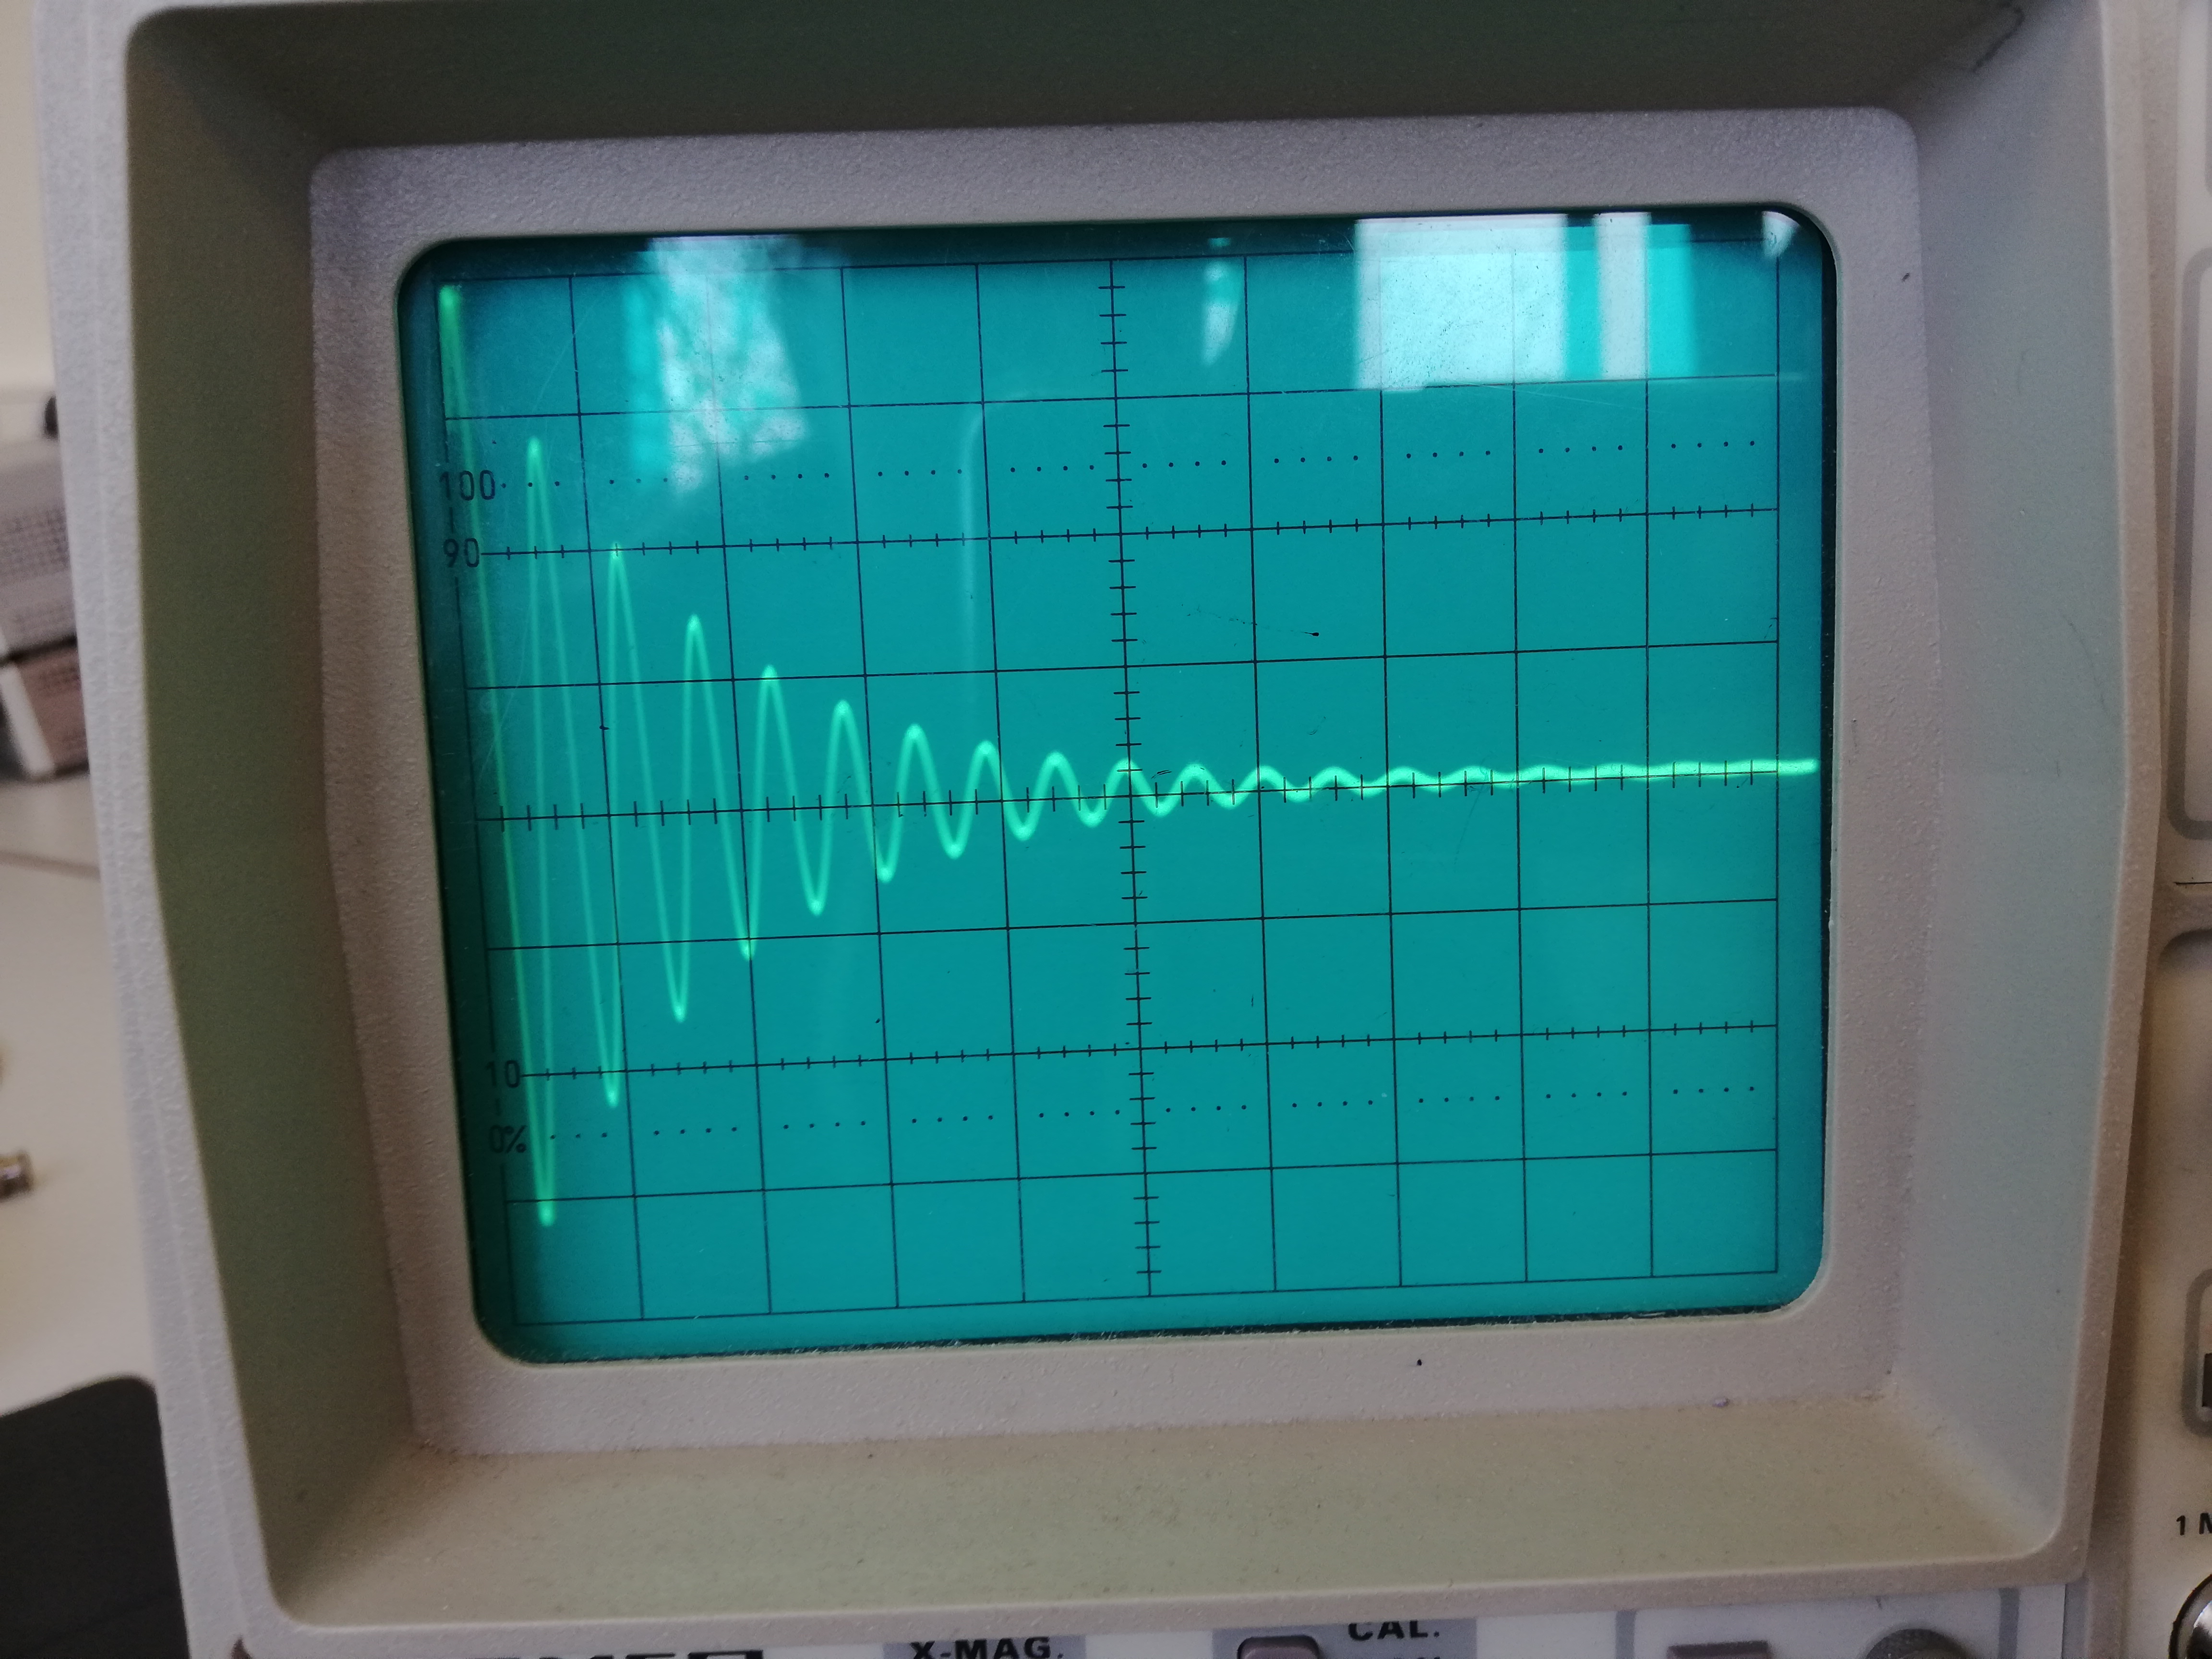
\includegraphics[width=13cm]{content/Auswertung.jpg}
  \caption{Kondensatorspannung in Abhängigkeit der Zeit beim gedämpften Schwingkreis}
  \label{fig:a1}
\end{figure}

\begin{table}[H]
  \centering
  
  \csvreader[tabular=c|c,
  head=false, 
  table head= $t\:/\:\si{\micro\second}$ & $U_C\:/\:\si{\volt}$ \\
  \midrule,
  late after line= \\]
  {daempfung.csv}{1=\eins, 2=\zwei}{$\num{\eins}$ & $\num{\zwei}$}
  
  \caption{Kondensatorspannung in Abhängigkeit der Zeit beim gedämpften Schwingkreis}
  \label{tab:a}
\end{table}

\noindent Aus Abbildung \ref{fig:a1} wurden 12 Wertepaare
abgelesen und in Tabelle \ref{tab:a} aufgelistet. Um
die Abklingduaer $T_{ex}$ zu bestimmen wurde nun zunächst
eine lineare Ausgleichsrechnung durchgeführt. Dabei
wurde eine Lineare Ausgleichsgerade mit Matplotlib
erstellt, welche in Abbildung \ref{fig:b} zu sehen ist.
Die Steigung

\begin{equation*}
  m=(-0,01032\pm0,00029)\cdot 10^{-3}\,\si{\second}^{-1}
\end{equation*}

\noindent dieser Geraden entspricht dem Faktor im Exponenten in Gleichung \ref{eq:a1},
da $U_C(t)$ proportional zu $I(t)$ ist. Die Abklingdauer
kann nach Gleichung \ref{eq:a2} durch das 
Inverse des Betrags der Steigung als 

\begin{equation*}
  T_{ex}=(96,9\pm2,7)\cdot10^{3}\,\si{\second}
\end{equation*}

\noindent berechnet werden. Mit der Abklingdauer kann nun eine nichtlineare Ausgleichskurve
erstellt werden, die der Einhüllenden in Abbildung \ref{fig:a1}
entspricht. Die Ausgleichsgerade ist mit den abgelesenen
Messwerten in Abbilung \ref{fig:a} zu sehen.

\begin{figure}[H]
  \centering
  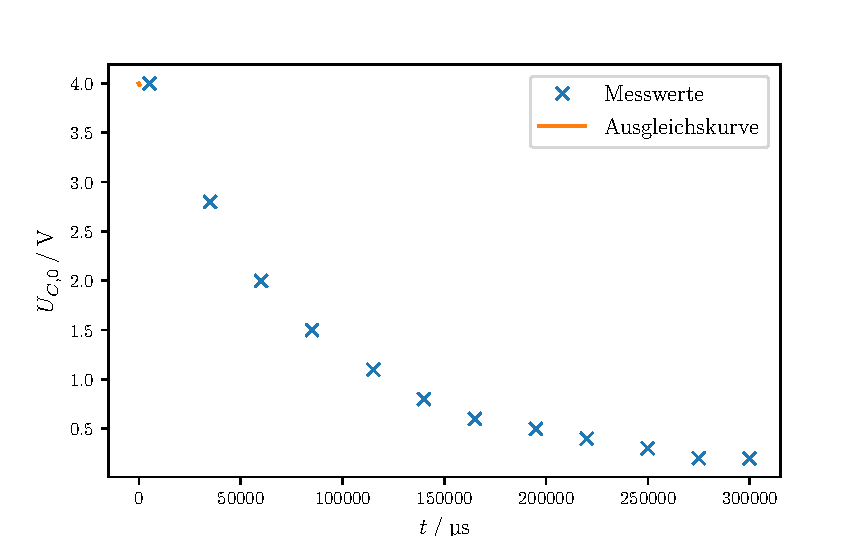
\includegraphics{build/plot1.pdf}
  \caption{Amplitudenmaximum der Kondensatorspannung eines RLC-Kreises in Abhängigkeit der Zeit}
  \label{fig:a}
\end{figure}

\begin{figure}[H]
  \centering
  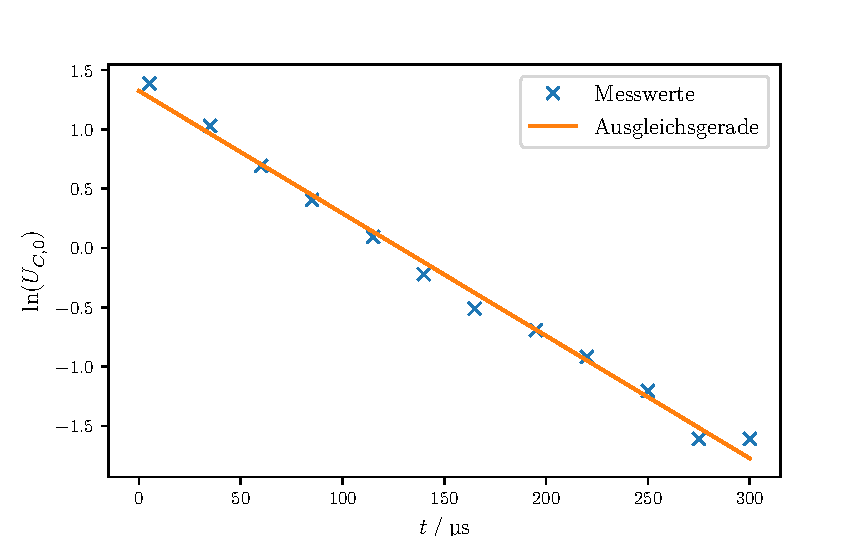
\includegraphics{build/plot1-1.pdf}
  \caption{Linearisierte Darstellung der Amplitudenmaxima der Kondensatorspannung eines RLC-Kreises in Abhängigkeit der Zeit}
  \label{fig:b}
\end{figure}

\noindent Der Dämpfungswiderstand $R_{eff}$ ergibt sich duch
Zusammenhang \ref{eq:a2} als

\begin{equation*}
  R_{eff}=(0,07224\pm0,0021)\cdot10^{-3}\,\si{\ohm}
\end{equation*}

\noindent Die Abweichung zum eigentlichen Widerstandwert $R=(30,3 \pm 0,1)\,\si{\ohm}$
lässt sich nicht allein durch den Innenwiderstand des Generators erklären,
welcher $R_G=600\,\si{\ohm}$ beträgt, denn damit würde $R=(30,3\pm0,1)\,\si{\ohm} + 600\,\si{\ohm}$





\subsection{Aperiodischer Grenzfall}
Bei der Messung nach \ref{sec:ap}
ergab sich für $R_{ap}$ ein Wert von

\begin{equation*}
  R_{ap}=1,4\,\si{\kilo\ohm}
\end{equation*}

\noindent Mit Gleichung (REFERENZ) lässt sich $R_{ap}$ 
als

\begin{equation*}
  R_{ap}=(1,673\pm0,004)\,\si{\kilo\ohm}
\end{equation*}

\noindent berechnen. Beim Verglich mit dem Messwert fällt 
auf, dass sich die Abweichung durch den nicht beachteten
Innenwiderstand $R_G=600\,\si{\ohm}$ des Generators erklären lässt.




\subsection{Frequenzabhängigkeit der Kondensatorspannung}

\begin{table}[H]
  \centering
  
  \csvreader[tabular=c|c,
  head=false, 
  table head= $\omega\:/\:\si{\kilo\hertz}$ & $U_C\:/\:\si{\volt}$ \\
  \midrule,
  late after line= \\]
  {tabelle2.csv}{1=\eins, 2=\zwei}{$\num{\eins}$ & $\num{\zwei}$}
  
  \caption{Frequenzabhängigkeit der Kondensatorspannung bei einer erzwungenen Schwingung}
  \label{tab:b}
\end{table}

\begin{figure}[H]
  \centering
  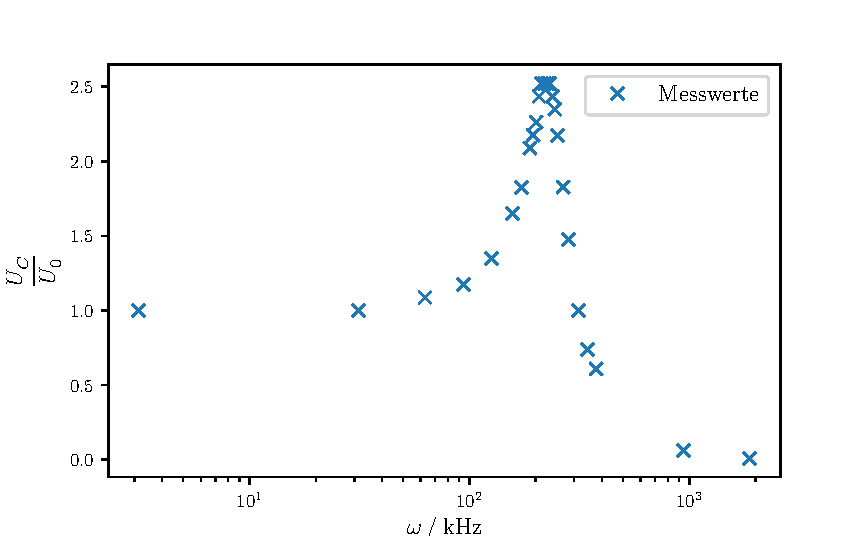
\includegraphics{build/plot2.pdf}
  \caption{Frequenzabhängigkeit der Kondensatorspannung bei einer erzwungenen Schwingung}
  \label{fig:c}
\end{figure}


\noindent Die Messwerte aus Tabelle \ref{tab:b} werden
in Abbildung \ref{fig:c} dargestellt. Dabei ist $U_0$ 
der gemessene Wert $U_0=2,3\,\si{\volt} $ der Generatorspannung. Die Resonanzüberhöhung
lässt sich als

\begin{equation*}
  q=2,52
\end{equation*}

\noindent ablesen. Dieser lässt sich mit dem nach Gleichung
\ref{eq:b1} als 

\begin{equation*}
  q=0,9599\pm0,0024
\end{equation*}
\noindent errechneten Wert vergleichen. Für diesen wurde
nun $R=(271,6\pm0,1)\,\si{\ohm} + 600\,\si{\ohm}$ angenommen.
In Abbildung \ref{fig:g} ist der Bereich
um die Resonanzfrequenz linear dargestellt.
\begin{figure}[H]
  \centering
  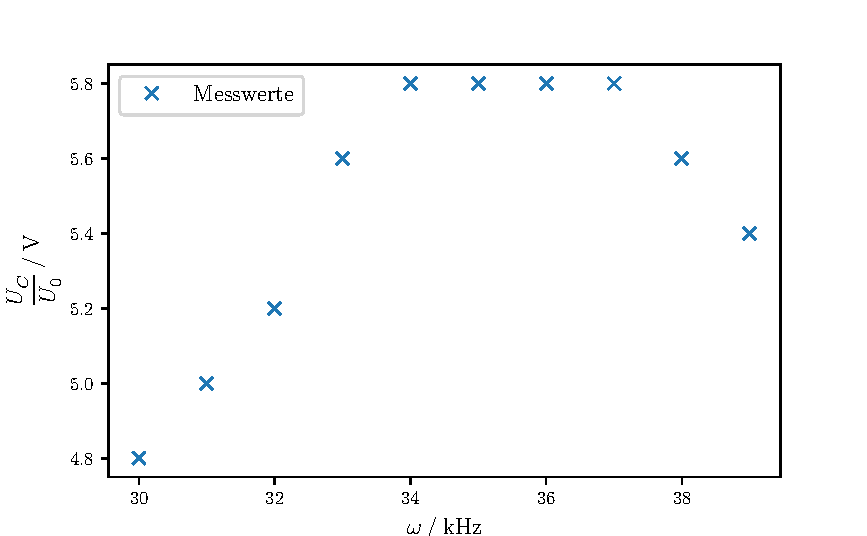
\includegraphics{build/plot3.pdf}
  \caption{Frequenzabhängigkeit der Kondensatorspannung bei einer erzwungenen Schwingung in Nähe der Resonanz}
  \label{fig:g}
\end{figure}



\subsection{Frequenzabhängigkeit der Phasenverschiebung zwischen Kondensator- und Generatorspannung}

\begin{table}[H]
  \centering
  
  \csvreader[tabular=c|c|c|c,
  head=false, 
  table head= $\omega\:/\:\si{\kilo\hertz}$ & $a\:/\:\si{\micro\second}$ & $b\:/\:\si{\micro\second}$ & $\phi$ \\
  \midrule,
  late after line= \\]
  {tabelle1.csv}{1=\eins, 2=\zwei, 3=\drei, 4=\vier}{$\num{\eins}$ & $\num{\zwei}$ & $\num{\drei}$ & $\num{\vier}$}
  
  \caption{Frequenzabhängigkeit der Phasenverschiebung zwischen Kondensator- und Generatorspannung}
  \label{tab:g}
\end{table}

\begin{figure}[H]
  \centering
  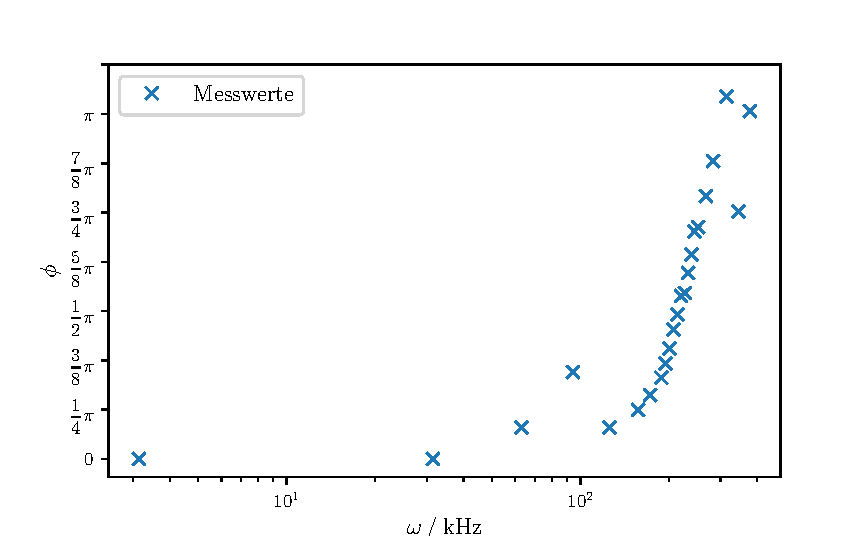
\includegraphics{build/plot4.pdf}
  \caption{Frequenzabhängigkeit der Phasenverschiebung zwischen Kondensator- und Generatorspannung}
  \label{fig:j}
\end{figure}
\noindent Die Messwerte aus Tabelle \ref{tab:g} werden in Abbildung
\ref{fig:j} dargestellt. Da bei der Durchführung nicht zwischen
positiver und negativer Phasenverschiebung unterschieden wurde,
werden alle Werte positiv dargestellt, obwohl Gleichung \ref{eq:ll}
zeigt, dass die Funktion bei kleinen Frequenzen negative Werte annimmt.
In Abbildung \ref{fig:i} ist
der Bereich um die Resonanzfrequenz linear dargestellt.
Diese lässt sich an der Stelle $\pi/2$ als

\begin{equation*}
  \omega_{res}=239\,\si{\kilo\hertz}
\end{equation*}


\noindent ablesen. Im Vergleich zum, durch Gleichung \ref{eq:res},
gerechneten Wert

\begin{equation*}
  \omega_{res}=(161,7\pm0,7)\,\si{\kilo\hertz}
\end{equation*}

\noindent fällt auf, dass der Theoriewert weit unter dem gemessenen Wert liegt.
Auch hier wurde $R=(271,6\pm0,1)\,\si{\ohm} + 600\,\si{\ohm}$ angenommen.
\begin{figure}[H]
  \centering
  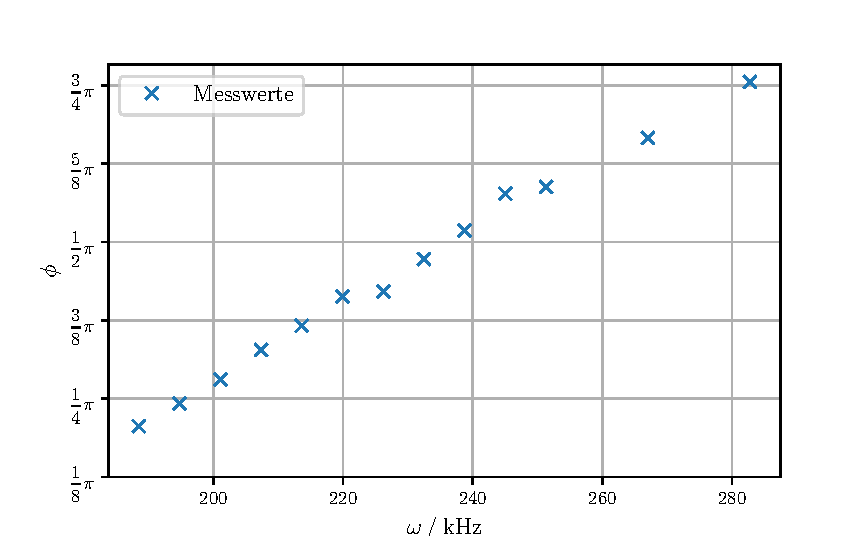
\includegraphics{build/plot5.pdf}
  \caption{Frequenzabhängigkeit der Phasenverschiebung zwischen Kondensator- und Generatorspannung in Nähe der Resonanz}
  \label{fig:i}
\end{figure}
\noindent $\omega_1$ liegt bei $\pi/4$ und entspricht
somit dem Messwert

\begin{equation*}
  \omega_1=195\,\si{\kilo\hertz}.
\end{equation*}


\noindent $\omega_1$ liegt bei $\pi \cdot 3/4$ und entspricht
somit dem Messwert

\begin{equation*}
\omega_2=283\,\si{\kilo\hertz}.
\end{equation*}
\noindent Diese Werte können mit den beiden aus Gleichung \ref{eq:bb}
errechneten Werten 

\begin{equation*}
  \omega_1=(145\pm0,4)\,\si{\kilo\hertz}
\end{equation*}
\begin{equation*}
  \omega_2=(394\pm0,9)\,\si{\kilo\hertz}
\end{equation*}

\noindent verglichen werden.


